\documentclass[11pt,a4paper,oldfontcommands,oneside]{memoir}
\usepackage[utf8]{inputenc}
\usepackage{microtype}
\usepackage[dvips]{graphicx}
\usepackage{xcolor}
\usepackage{times}
\usepackage{graphicx}
\usepackage[spanish]{babel}
\usepackage[
breaklinks=true,colorlinks=true,
%linkcolor=blue,urlcolor=blue,citecolor=blue,% PDF VIEW
linkcolor=black,urlcolor=black,citecolor=black,% PRINT
bookmarks=true,bookmarksopenlevel=2]{hyperref}

\usepackage{geometry}
% PDF VIEW
% \geometry{total={210mm,297mm},
% left=25mm,right=25mm,%
% bindingoffset=0mm, top=25mm,bottom=25mm}
% PRINT
\geometry{total={210mm,297mm},
left=20mm,right=20mm,
bindingoffset=10mm, top=25mm,bottom=25mm}

\OnehalfSpacing
%\linespread{1.3}

%%% CHAPTER'S STYLE
\chapterstyle{bianchi}
%\chapterstyle{ger}
%\chapterstyle{madsen}
%\chapterstyle{ell}
%%% STYLE OF SECTIONS, SUBSECTIONS, AND SUBSUBSECTIONS
\setsecheadstyle{\Large\bfseries\sffamily\raggedright}
\setsubsecheadstyle{\large\bfseries\sffamily\raggedright}
\setsubsubsecheadstyle{\bfseries\sffamily\raggedright}


%%% STYLE OF PAGES NUMBERING
%\pagestyle{companion}\nouppercaseheads 
%\pagestyle{headings}
%\pagestyle{Ruled}
\pagestyle{plain}
\makepagestyle{plain}
\makeevenfoot{plain}{\thepage}{}{}
\makeoddfoot{plain}{}{}{\thepage}
\makeevenhead{plain}{}{}{}
\makeoddhead{plain}{}{}{}


\maxsecnumdepth{subsection} % chapters, sections, and subsections are numbered
\maxtocdepth{subsection} % chapters, sections, and subsections are in the Table of Contents


%%%---%%%---%%%---%%%---%%%---%%%---%%%---%%%---%%%---%%%---%%%---%%%---%%%

\begin{document}

%%%---%%%---%%%---%%%---%%%---%%%---%%%---%%%---%%%---%%%---%%%---%%%---%%%
%   TITLEPAGE
%
%   due to variety of titlepage schemes it is probably better to make titlepage manually
%
%%%---%%%---%%%---%%%---%%%---%%%---%%%---%%%---%%%---%%%---%%%---%%%---%%%
\thispagestyle{empty}

{%%%
\sffamily
\centering
\Large

~\vspace{\fill}

\includegraphics[scale=1]{logo1.png} \\
{\huge 
\vspace{4cm}
Describir las características de cinemática directa e inversa de manipuladores paralelos
}
\vspace{2.5cm}

{\LARGE
Eduardo Robles Vázquez
}

\vspace{2.5cm}

Universidad Politécnica de la Zona Metropolitana de Guadalajara

\vspace{3.5cm}

Profesor: Carlos Enrique Morán Garabito

\vspace{\fill}

29 de Octubre de 2019

%%%
}%%%

\vspace{.5cm}
\hfill\break




\tableofcontents*

\clearpage

%%%---%%%---%%%---%%%---%%%---%%%---%%%---%%%---%%%---%%%---%%%---%%%---%%%
%%%---%%%---%%%---%%%---%%%---%%%---%%%---%%%---%%%---%%%---%%%---%%%---%%%

\chapter{Cinemática Directa.}

Utilizando la notación de Denavit y Hartenberg se puede expresar la posición y orientación del efector final del manipulador en función del desplazamiento de sus articulaciones. El desplazamiento articular es un ángulo ($\theta_i$) o una distancia ($d_i$), dependiendo del tipo de articulación.

Los robots paralelos donde el número de cadenas es estrictamente igual al número de GDL del efector final son llamados manipuladores paralelos completos. Hay dos casos de robots paralelos: planos, esféricos o espaciales. Un robot completamente paralelo plano tiene 3 GDL en su efector final, dos de traslación y uno de rotación. Un robot completamente paralelo con \textit{m} GDL posee \textit{m} cadenas unidas a su efector final. Si las cadenas son idénticas se puede utilizar la fórmula de Gruber's, aunque algunas veces esta fórmula puede tener errores debido a que no considera las relaciones geométricas entre las juntas.

Un manipulador paralelo se puede considerar como simétrico si se satisfacen las siguientes condiciones:

1. El número de cadenas es igual al número de grados de libertad de la plataforma móvil.

2.EL tipo y numero de juntos de todas las cadenas son iguales.

3.El número y la localización de las juntas activas en todas las cadenas son las mismas.

\section{Robots paralelos planos}

Para definir un cuerpo plano cartesiano se necesitan dos coordenadas y un ángulo, en el caso de los manipuladores paralelos planos de 2 grados de libertad solo se pueden describir por dos coordenadas ya sean cartesianas o polares y en el caso de manipuladores paralelos planos de 3 grados de libertad se pueden describir las dos coordenadas y la orientación.

\section{Robots paralelos planos de 2 GDL}

Los robots paralelos planos de 2 grados de libertad están formados por paralelogramos que permiten que el eslabón de salida permanezca en una orientación fija con respecto al eslabón de entrada, las ventajas son la capacidad de rotación altas. JX Liu, en 2003, presenta mecanismos paralelos que tienen amplias aplicaciones en robots industriales, simuladores, micro manipuladores, maquina denominadas de cinemática paralela, y cualquier otro dispositivo de manipulación en los que se necesitan alta capacidad de rotación y alta rigidez. Sobre todo, presenta nuevos conceptos de diseño de mecanismos paralelos, novedosos y la mejora de la capacidad de rotación de dichos sistemas.

En la \ref{Figure 1} se muestran algunas arquitecturas de manipuladores paralelos de 2 GDL. Presentados por Figielski, 2007, los cuales están formados por juntas rotaciones y juntas prismáticas.

\begin{figure}[htp]
\centering
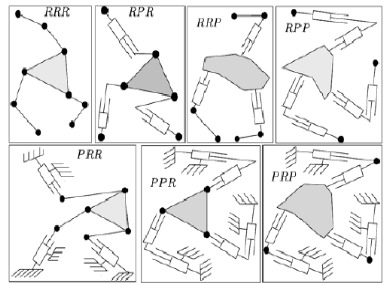
\includegraphics[scale=1.00]{1.jpg}
\caption{Robots paralelos de 2 GDL}
\label{Figure 1}
\end{figure}

\section{Robots paralelos de planos de 3 GDL}

En los manipuladores paralelos de 3 GDL, se asume que cada cadena cuenta con tres juntas y dos eslabones. Utilizando juntas rotacionales \textit{R} y juntas prismáticas \textit{P}. Cada una de las cadenas cinemáticas independientes se denota por un conjunto de tres letras que indican la sucesión de las juntas a partir de la tierra. Las combinaciones son, por tanto: \textit {RRR}, \textit {RPR}, \textit {PPR}, \textit {RRP}, \textit {PRP}, \textit {PPP}, la configuración \textit {PPP} presenta movimientos independientes. Si se asume que las tres cadenas cinemáticas son idénticas, se presentan todas las configuraciones posibles en la \ref {Figure 2}

\begin{figure}[htp]
\centering
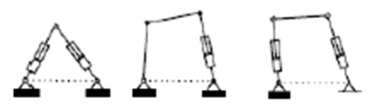
\includegraphics[width=8cm]{2.jpg}
\caption{Manipuladores paralelos planos de 3GDL}
\label{Figure 2}
\end{figure}

El plano paralelo plano está constituido por una plataforma móvil, conectada a tierra por tres cadenas cinemáticas independientes que tienen tres grados de libertad, independientes una articulación es accionada.

Las cadenas cinemáticas de cualquier manipulador plano completo pueden estar compuestas en cada cadena por cualquier secuencia de las juntas que se muestran en la \ref {Tabla 1}

\begin{center}
\begin{table}
\begin{tabular}{|c|c|c|c|c|c|}
\hline
	RRR & RRR & RRR & RPR & RPR & RPR\\
\hline
	RPP & RPP & PRR & PRR & PRR & PRP\\
\hline
	PRP & PPR & PPR & RRP & RRP & RRP\\
\hline
\end{tabular}
\caption{Cadenas cinemáticas robot 3GDL}
\label{Tabla 1}
\end{table}
\end{center}

Los manipuladores paralelos planos se definen por la secuencia que describe las tres cadenas cinemáticas, por ejemplo, Gosselin y Angeles en 1988, presentan el robot paralelo 3RRR que es el robot con tres cadenas cinemáticas RRR. Entre los investigadores que realizaron un extenso estudio sobre estos robots, se encuentran Kassner, Gosselin. Por otro lado, la síntesis dimensional ha sido abordad por Shikbodaie, 1987 y Arsenault, 2004, análisis de singularidades por Gosselin y espacio de trabajo Kumar, 1992. Lui, 200, Gao 2001, rigidez Kim, 2000.

\chapter{Cinemática inversa}

Para los manipuladores paralelos la cinemática inversa resulta ser más simple, en comparación con la cinemática directa.

En robots paralelos la cinemática inversa consiste en establecer el valor de las juntas activas y pasivas en función de las coordenadas del extremo del robot, las juntas activas son las juntas actuadas y las juntas pasivas son las que quedan en función de las juntas activas. Establecer la cinemática inversa es esencial para el control de la posición de los robots paralelos. EL mapeo de la cinemática, tiene interesantes ecuaciones algebraicas que tienen múltiples soluciones. La cinemática inversa de los manipuladores paralelos en general es idéntica a la de los manipuladores serie.



\bibliographystyle{plain}
\bibliography{bibliografia}


\end{document}

